\documentclass[12pt]{article}
\usepackage[margin=1in]{geometry}
\usepackage{amsmath}
\usepackage{amssymb}
\usepackage{graphicx}
\usepackage{subfig}
\usepackage{stmaryrd}
\usepackage{float}

\author{Kyler Little\vspace{-0.6cm}}
\title{Homework \#6: Machine Learning\vspace{-0.3cm}}
\date{April 20, 2018\vspace{-0.7cm}}

\begin{document}
	\maketitle
	\section*{Problem \#1}
	Let $A = U \Sigma V^T$ be the SVD of $A$, where $A \in R^{m\times n}$, $U \in R^{m\times m}$ and $V \in R^{n\times n}$
	are orthogonal matrices, $\Sigma = \text{diag}(\sigma_1 , \cdots, \sigma_r, 0, \cdots, 0)$, and $r = \text{rank}(A)$. Show that: \\
	(a) The first $r$ columns of $U$ are eigenvectors of $AA^T$ corresponding to nonzero eigenvalues. \\
	\begin{align*}
		AA^T &= U\Sigma V^T (U\Sigma V^T)^T \\
		&= U\Sigma V^T (V^T)^T\Sigma^T U^T \\
		&= U\Sigma \Sigma^T U^T \\
		&= U \left[\begin{array}{cc}
		\Sigma^{*2} & 0 \\
		0 & 0
		\end{array}\right] U^T
	\end{align*}
	Note that $\Sigma^{*2} = \text{diag}(\sigma_1^2 , \cdots, \sigma_r^2)$, and the transition from the second step to the third occurs because $V$ is an orthonormal matrix. Because $AA^T$ is symmetric (true for any matrix $A$), we see that the final equation is actually the eigen decomposition of $AA^T$. Therefore, the columns of $U$ are the eigenvectors of $AA^T$. Clearly, only the first $r$ columns of $U$ can possibly correspond to nonzero eigenvalues since the remaining diagonal entries of $\Sigma^2$ are zeros. But to prove this, we must show $(AA^T)_r$ is positive definite. This is relatively easy, using the knowledge of past homeworks. Given any $x \in R^r \ \text{s.t.}\  x \ne 0$, we have that $x^T(AA^T)_r x=(A^T x)^T A^T x = ||A^T x||^2 > 0$ for nonzero $x$. Therefore, we have that the eigenvalues of $(AA^T)_r$ are all positive and nonzero, so we are done.
	\\ \\
	(b) The first $r$ columns of $V$ are eigenvectors of $A^TA$ corresponding to nonzero eigenvalues. \\
	\begin{align*}
	A^T A &= (U\Sigma V^T)^T U\Sigma V^T \\
	&= (V^T)^T\Sigma^T U^T U\Sigma V^T \\
	&= V\Sigma^T \Sigma V^T \\
	&= V \Sigma^{*2} V^T
	\end{align*}
	As we can see, a nearly identical argument can be made for this case. Clearly, the last equation is an eigen decomposition for $A^TA$. It only needs to be proved that the diagonal entries of $\Sigma^{*2}$ are strictly positive. Similar to the part (a), we have that given any $x \in R^r \ \text{s.t.}\  x \ne 0$, $x^T(A^TA)_r x=(Ax)^T Ax = ||Ax||^2 > 0$ for nonzero $x$. Therefore, we have that the eigenvalues of $(A^TA)_r$ are all positive and nonzero, so we are done once more.
	
	\section*{Problem \#2}
	Given a symmetric matrix $A \in R^{3\times 3}$, suppose its eigen-decomposition can be written as:
	\begin{equation*}
		A =
		\left(
		\begin{array}{ccc}
		u_{11} & u_{12} & u_{13} \\
		u_{21} & u_{22} & u_{23} \\
		u_{31} & u_{32} & u_{33}
		\end{array}
		\right)
		\left(
		\begin{array}{ccc}
		3 & 0 & 0 \\
		0 & -2 & 0 \\
		0 & 0 & 1
		\end{array}
		\right)
		\left(
		\begin{array}{ccc}
		u_{11} & u_{21} & u_{31} \\
		u_{12} & u_{22} & u_{32} \\
		u_{13} & u_{23} & u_{33}
		\end{array}
		\right)
	\end{equation*}
	What is the singular value decomposition of this matrix?
	\\
	Firstly, note that the decomposition is already quite close to the SVD. The only issue is that $-2$ should be positive, but otherwise, the magnitudes of the eigenvalues are nonincreasing and all greater than zero. Thus, a nice trick we can apply is to note that $AA^T=U\Lambda U^T U\Lambda U^T = U \Lambda^2 U^T$ (recall $U^T U = I$ and $\Lambda$ is a diagonal matrix), which is a singular value decomposition of $A A^T$. Because $A$ is symmetric, we have that $A^T A = AA^T$. Knowing this, we can see that the only thing that changes between the eigen-decomposition for $A$ and the SVD for $A A^T$ is actually the central matrix ($\Lambda \ \text{versus}\  \Lambda^2$). Thus, to obtain the SVD for $A$, we must ensure that the sign of the singular values is kept positive. We can do this by putting the sign of each eigenvalue on to the corresponding column vector in $U$ and then making all eigenvalues positive by taking their absolute values. In other words, let $A=\sum_{i=1}^{3}\text{sign}(\lambda_i)u_i |\lambda_i|u^T$.
	Therefore, the SVD for $A$ is:
	\begin{equation*}
	A =
	\left(
	\begin{array}{ccc}
	u_{11} & -u_{12} & u_{13} \\
	u_{21} & -u_{22} & u_{23} \\
	u_{31} & -u_{32} & u_{33}
	\end{array}
	\right)
	\left(
	\begin{array}{ccc}
	3 & 0 & 0 \\
	0 & 2 & 0 \\
	0 & 0 & 1
	\end{array}
	\right)
	\left(
	\begin{array}{ccc}
	u_{11} & u_{21} & u_{31} \\
	u_{12} & u_{22} & u_{32} \\
	u_{13} & u_{23} & u_{33}
	\end{array}
	\right)
	\end{equation*}
	\section*{Problem \#3}
	Given a data matrix $X = \left[
	\begin{array}{cccc}
	x_1, & x_2, & \cdots & x_n
	\end{array}
	\right] \in R^{p \times n}$ consisting of $n$ data points, and each data point is $p$-dimensional, \\
	$\bullet$ Outline the procedure for computing the PCA of X.\\
	PCA is a strategy for reducing the dimension of data through the reduction of features (rather than feature selection). The strategy to do this, at a high level viewpoint, is to simply use a linear transformation on each data point to produce a ``reduced" data point with fewer dimensions (but roughly the same qualities). The important part of PCA is in how it determines to transform each data point. PCA does this by computing the eigenvectors of the covariance matrix of the input data matrix. But before getting into the mechanics of this, I will establish some notation. Given input data matrix $X \in R^{p \times N}$, we would like to reduce the dimensionality of each column of $X$ to $d$ (from $p$). We can do this via a linear transformation $G \in R^{p \times d}: X \rightarrow Z = G^T X \in R^{d \times N}$, where $Z$ is the transformed input data matrix. Now, we can begin to discuss the mechanics. If the first $d$ eigenvectors form matrix $U_d$, then the matrix product $U_d^T X$ will produce the transformed input data matrix. To find the eigenvectors, we first need the matrix itself. The covariance matrix of $X$ is simply $\frac{1}{2}\tilde{X}\tilde{X}^T$, where $\tilde{X}=X-\bar{x}1_{1\times N}$ and $\bar{x} = \frac{1}{N}\sum_{i=1}^{N} x_i$ (note that $x_i$ is the $i$th column vector of X). To compute $\tilde{X}$'s eigenvectors, we compute its SVD: $\text{SVD}(\tilde{X}) = U\Sigma V^T$. Now, we simply take the first $d$ columns of $U$, and let these form the matrix $G$, and we are done. We now have $G$ such that $G^T X = Z \in R^{d \times N}$.
	\\
	$\bullet$ State what is the “minimum reconstruction error” property of PCA. \\
	The minimum reconstruction error property states that the PCA minimizes the error in reconstructing a matrix from its reduced form (i.e. no better method exists). In mathematical terms, PCA minimizes the Frobenius norm of $X - GG^T X$.
	\\
	$\bullet$ Prove the minimum reconstruction error property of PCA by using the best low-rank
	approximation property of SVD. \\
	Basically what we need to show is that $GG^T X$ is equal to the best $d$-rank approximation of $X$, and this will suffice. To start, note that $GG^TX = U_dU_d^TX$, meaning that we are trying to prove that $U_dU_d^TX = U_d\Sigma_dV_d^T$. 
	First, we note that $X$ can be represented by SVD: $X=U\Sigma V^T$, so we substitute this in. Therefore, $U_dU_d^TX = U_dU_d^T U\Sigma V^T$. Next we note that $U_d^TU=I_{d \times N}$, since $U$ and all of its submatrices (by column) are orthonormal. Thus, we now have $U_d I_{d \times N} (\Sigma V^T)$, which equals $U_d\Sigma_dV_d^T$, and we are done.
	\section*{Problem \#4}
	Use the similarity matrix in Table 1 to perform single
	(MIN) and complete (MAX) link hierarchical clustering. Show your results by drawing a
	dendrogram. The dendrogram should clearly show the order in which the points are merged.
	\begin{table}[H]
		\centering
		\caption{Similarity Matrix}
		\begin{tabular}{c|c|c|c|c|c}
			& \textbf{p1} & \textbf{p2} & \textbf{p3} & \textbf{p4} & \textbf{p5} \\
			\hline
			p1 & 1.00 & 0.10 & 0.41 & 0.55 & 0.35 \\
			p2 & 0.10 & 1.00 & 0.64 & 0.47 & 0.98 \\
			p3 & 0.41 & 0.64 & 1.00 & 0.44 & 0.85 \\
			p4 & 0.55 & 0.47 & 0.44 & 1.00 & 0.76 \\
			p5 & 0.35 & 0.98 & 0.85 & 0.76 & 1.00 \\
			\hline
		\end{tabular}
	\end{table}
	MIN: Clearly in the first round, we merge $p2$ and $p5$ since these are the closest. Then we merge $p2/p5$ and $p3$. Next, we merge $p2/p3/p5$ and $p4$. Lastly, we merge $p2/p3/p4/p5$ and $p1$.
	\\
	MAX: Weirdly enough, this actually produces the same results. We obviously have the same starting merge ($p2$ and $p5$) since this merge would have the smallest diameter. The next merge with the smallest diameter is: $p2/p5$ and $p3$, with diameter $1.00-0.64$. The other options would have been $p2/p5$ and $p1$ with diameter $1.00-0.10$, $p2/p5$ and $p4$ with diameter $1.00-0.47$, $p1$ and $p4$ with diameter $1.00-0.55$, $p1$ and $p3$ with diameter $1.00-0.41$, or $p4$ and $p3$ with diameter $1.00-0.44$. We can follow a similar process to determine the last two merges. This results in the exact same merges as the MIN method.
	\\
	Since the merges are identical, I drew only one diagram.
	\begin{figure}[H]
		\begin{center}
			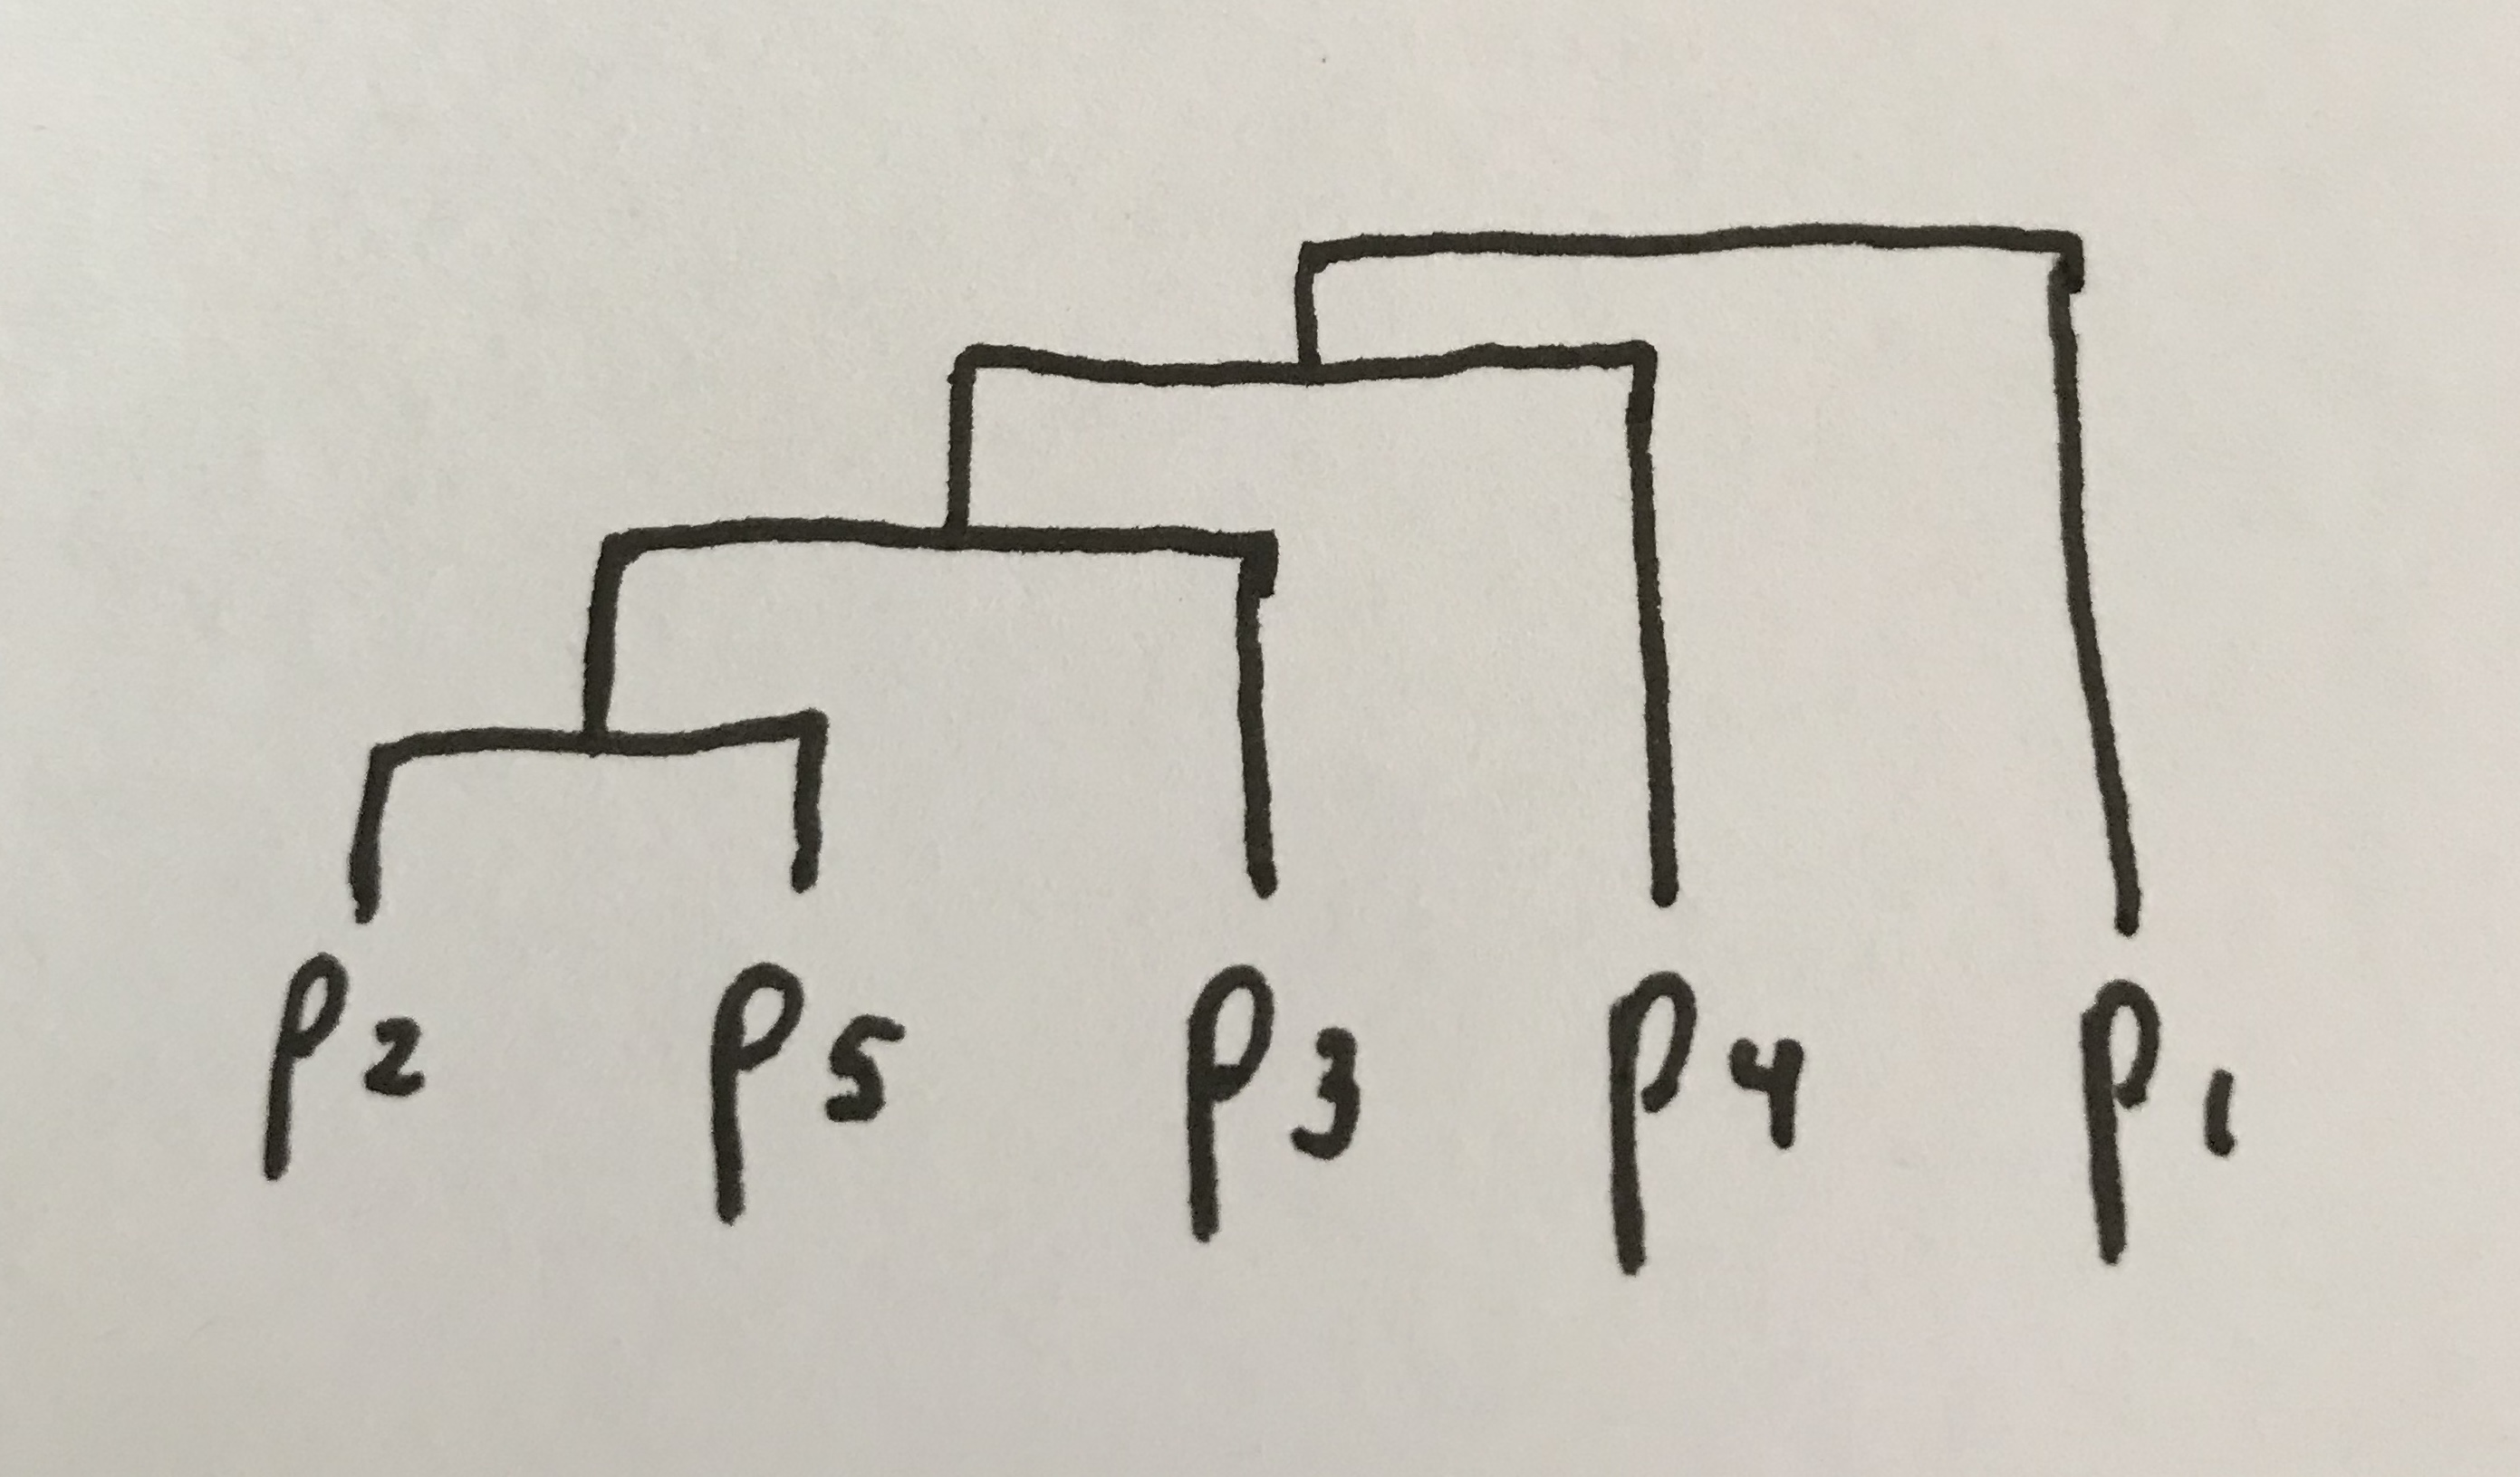
\includegraphics[width=300pt]{dendrogram.jpg}
			\caption{The resulting dendrogram using single and complete hierarchical clustering}
			\label{fig:dendro}
		\end{center}
	\end{figure}
	\section*{Problem \#5}
	Summarize results of PCA implementation and attach images. \\
	In the coding portion, we use PCA on a set of images of handwritten digits-- the same dataset as in past assignments. This, of course, reduces the dimension of the images; then we reconstruct the original images using the best low-rank approximation of each image for varying ranks (10, 50, 100, 200). The results are displayed for two particular images in Figures 2 and 3 below.
	\begin{figure}[H]
		\centering
		\subfloat[10 principal components]{{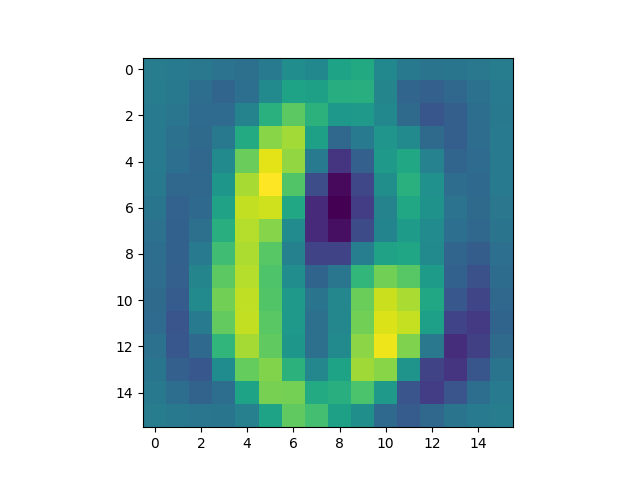
\includegraphics[width=6cm]{img1_comp10.png} }}
		\subfloat[50 principal components]{{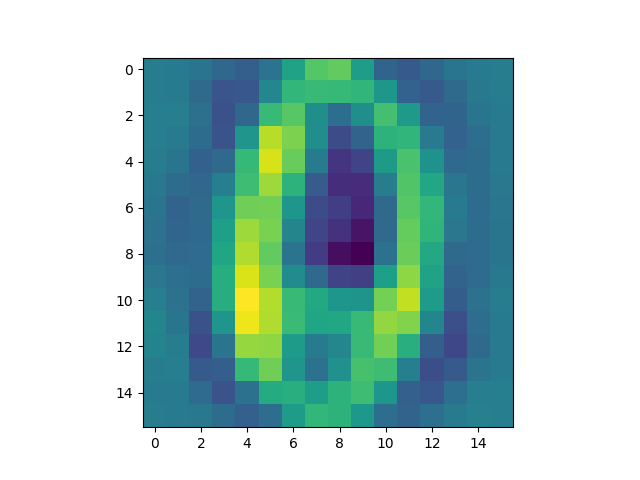
\includegraphics[width=6cm]{img1_comp50.png} }}
	\end{figure}
	\begin{figure}[H]
		\centering
		\subfloat[100 principal components]{{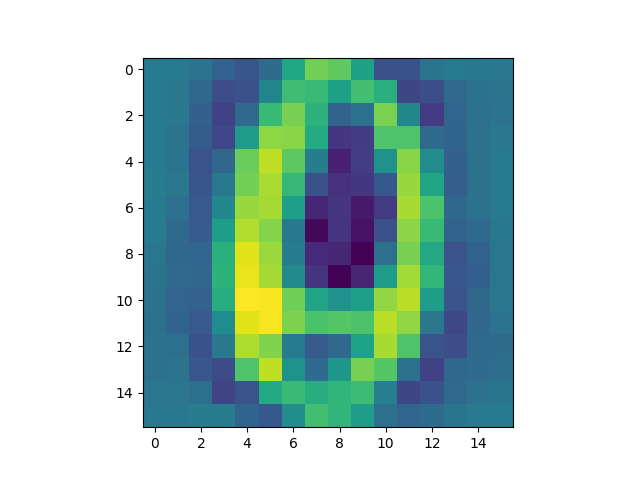
\includegraphics[width=6cm]{img1_comp100.png} }}
		\subfloat[200 principal components]{{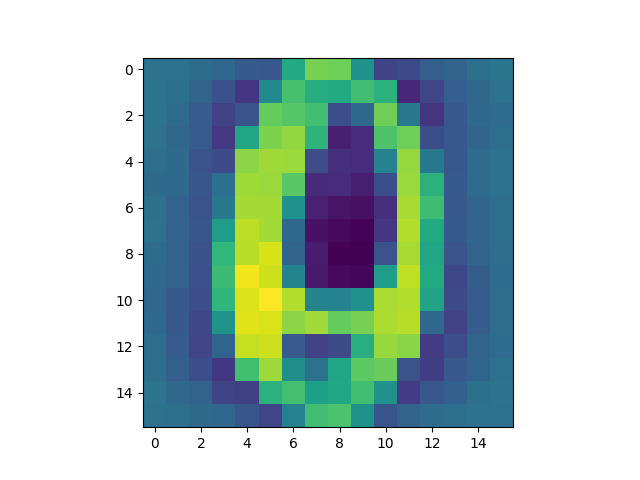
\includegraphics[width=6cm]{img1_comp200.png} }}
		\caption{Using PCA, we reconstruct the original image using the stated number of principal components.}
	\end{figure}
	\begin{figure}[H]
		\centering
		\subfloat[10 principal components]{{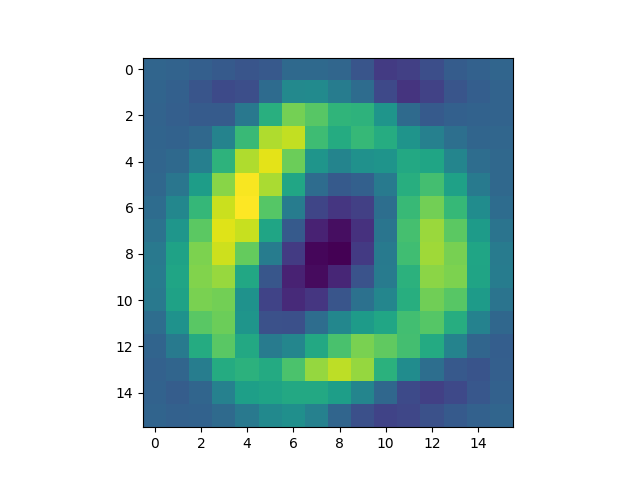
\includegraphics[width=6cm]{img2_comp10.png} }}
		\subfloat[50 principal components]{{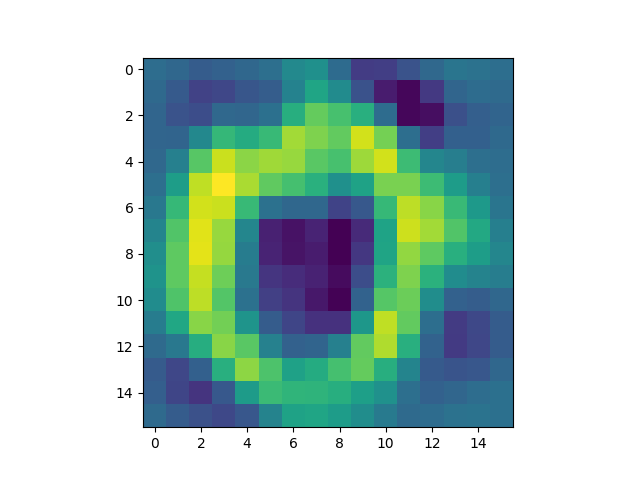
\includegraphics[width=6cm]{img2_comp50.png} }}
	\end{figure}
	\begin{figure}[H]
		\centering
		\subfloat[100 principal components]{{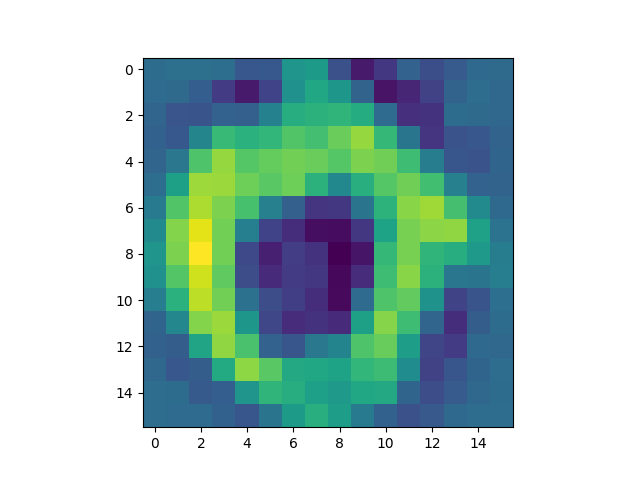
\includegraphics[width=6cm]{img2_comp100.png} }}
		\subfloat[200 principal components]{{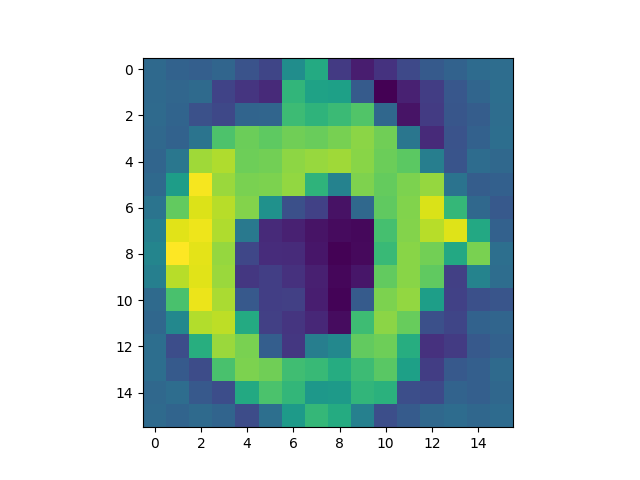
\includegraphics[width=6cm]{img2_comp200.png} }}
		\caption{Using PCA, we reconstruct the original image using the stated number of principal components.}
	\end{figure}
	As we can see from the figures, the quality of the reconstruction increases as the number of principal components is increased. This makes sense because we're not removing as many dimensions from our data. However, it's important to note that even the extremely low-rank approximations of the images are still quite good. It's still nearly possible to tell which digits the images represent, despite transforming to extremely low dimension and then back.
	
	
\end{document}